% !TEX root =  ../thesis.tex

In this chapter the results of our investigation are presented. We illustrate the quantitative results deriving from an automated analysis of several application on the Play Store; subsequently, we present a qualitative analysis and observation about the experiment.

\section{Quantitative results}
\label{sec:results}
In this section we present a metric used to evaluate the compliance of an application w.r.t. its privacy policy and we expose the quantitative results in terms of such metric.

\subsection{Metric definition}
\label{sec:metric}
First, we manually assign to each privacy-related permission a score from 1 to 3, representing the severity of its potential impact on the user's privacy, where 1 signifies a permission with low impact and 3 signifies a permission carrying a very high danger.

Such scores are defined by us, in accordance with observations and existing literature on permission analysis,
and are shown in \autoref{tab:permission-scores}.

\begin{table}[ht]
    \caption{PERMISSION IMPACT SCORES}
    \label{tab:permission-scores}
    \centering
    \begin{tabular}{clc}
        \toprule
            \#   & Permission impact scores \\
            \midrule
                1  & INTERNET                       &   3 \\
                2  & READ\_EXTERNAL\_STORAGE        &   2 \\
                3  & WRITE\_EXTERNAL\_STORAGE       &   2 \\
                4  & ACCESS\_WIFI\_STATE            &   1 \\
                5  & READ\_PHONE\_STATE             &   3 \\
                6  & GET\_ACCOUNTS                  &   3 \\
                7  & ACCESS\_COARSE\_LOCATION      	&   3 \\
                8  & GET\_TASKS                     &   1 \\
                9  & ACCESS\_FINE\_LOCATION         &   3 \\
                10 & READ\_LOGS                     &   1 \\
                11 & RECORD\_AUDIO                  &   2 \\
                12 & READ\_CONTACTS                 &   3 \\
        \bottomrule
    \end{tabular}
\end{table}

Secondly, we use the scores to compute a weighted sum of the number of permissions that lack an explicit mention in the privacy policy.

\begin{align}
\label{eq:goodness-metric}
	\sum\limits_{i=1}^n &= w_i p_i \\
	w_i &= \text{ score of the} i^{th} \text{permission} \\
	%
	p_i &=
	\begin{cases}
		& 0 \text{ if the permission is mentioned in the privacy policy} \\
		& 1 \text{ otherwise}
	\end{cases}
\end{align}

The final result is a metric estimating the compliance of an Android application to its own privacy policy. The lower the score, the more compliant the application.

We the analysis on the same 4300 applications used to generate the list of most used permissions, and the results are shown in \autoref{fig:results}

\begin{figure}[t]
\centering
     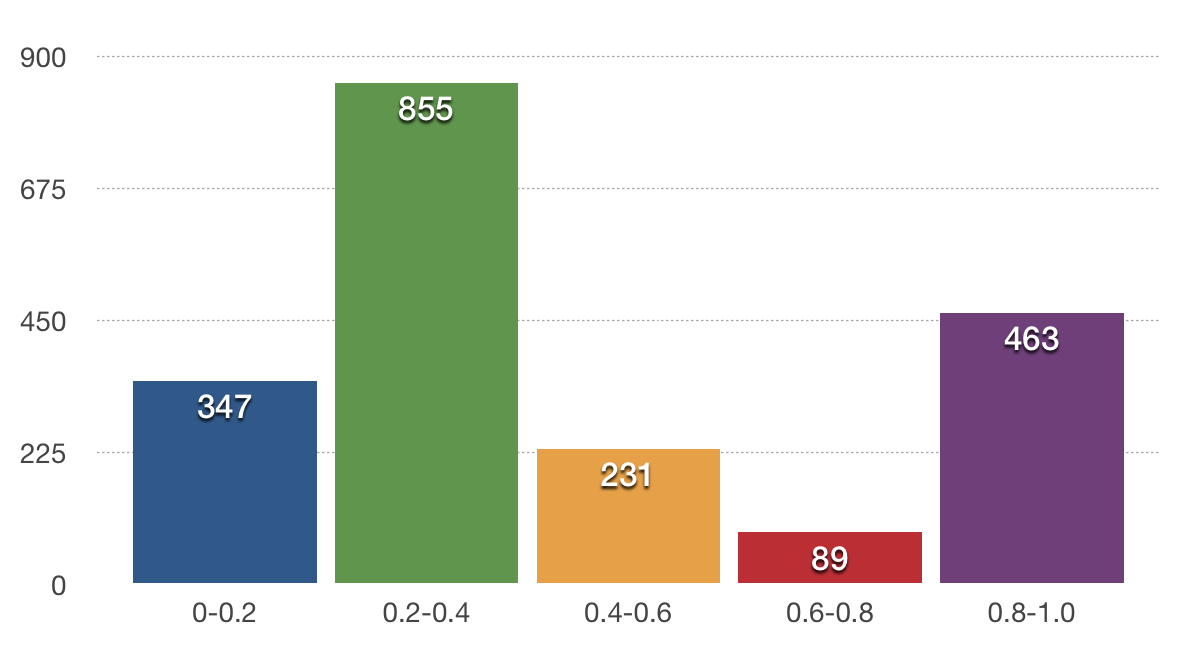
\includegraphics[width=0.9\textwidth]{images/results}
      \caption{Quantitative results (over 4300 applications, December 7, 2013)}
      \label{fig:results}
\end{figure}

\section{Qualitative results}
\label{sec:qualitative-results}
Out of the thousands of applications analyzed, we now focus our attention on a few notable cases.

\section{Case study: Shopkick}
Shopkick is a popular shopping rewards app and is known \cite{shopkick-lifehacker} to require some sensitive permissions that should worry any user of this app. \autoref{tab:shopkick-permissions} shows the complete list of permissions of the Android application.

\begin{table}[ht]
    \caption{SHOPKICK APP PERMISSIONS}
    \label{tab:shopkick-permissions}
    \centering
    \begin{tabular}{l}
        \toprule
            Permissions \\
            \midrule
                INTERNET \\
                ACCESS\_NETWORK\_STATE \\
                ACCESS\_COARSE\_LOCATION \\
                ACCESS\_FINE\_LOCATION \\
                READ\_PHONE\_STATE \\
                WRITE\_EXTERNAL\_STORAGE \\
                ACCESS\_WIFI\_STATE \\
                RECORD\_AUDIO \\
                CAMERA \\
                FLASHLIGHT \\
                VIBRATE \\
                BLUETOOTH \\
                GET\_ACCOUNTS \\
                RECEIVE\_BOOT\_COMPLETED \\
                READ\_CONTACTS \\
                CALL\_PHONE \\
                WAKE\_LOCK \\
                READ\_EXTERNAL\_STORAGE \\
                READ\_CALL\_LOG \\
        \bottomrule
    \end{tabular}
\end{table}

We can immediately spot a few permissions with a very high impact score, for example \texttt{RECORD\_AUDIO}, \texttt{CAMERA} and \texttt{ACCESS\_FINE\_LOCATION}.

\texttt{RECORD\_AUDIO} grants the application the ability to access the device microphone to record audio, without any explicit consent by the user other than installing the app itself. This means that the app is virtually enabled to record audio at any time, with no possibility of being disabled. Especially in combination with the \texttt{RECEIVE\_BOOT\_COMPLETED} permission, which allows the app to be launched when the phone has booted, and the \texttt{INTERNET} permission, which enables sending data over the Internet, this is considerably worrying: the application could easily start itself as soon as the phone has been turned on, constantly record any sound going through the device's microphone and finally send everything over the Internet to a remote server, where the content can be stored and accessed in a later time.

To make things worse, the application also requests the permission \texttt{ACCESS\_FINE\_LOCATION}, meaning that the audio recording can be triggered according to the user's location, perhaps the workplace, home or other sensitive locations.

It is not hard to see how these capabilities can turn the app into a roving spyware, i.e. an application with whose hidden purpose is eavesdropping and spying on the device owners, as well as the people they have contacts with.

Further investigations reveal how the app apparently uses the device's microphone in order to validate the physical location of the user in a store. According to the New York Times, \emph{``The app knows someone is in a store by listening for an audio transmitter placed in each participating store; the phone's microphone picks up the signal, which people cannot hear.''}\cite{shopkick-nyt}.

We can formalize a subset of this situation in terms of the representation previously discussed in \autoref{chap:intro}.
\begin{itemize}
    \item The permission \texttt{RECORD\_AUDIO} ($P_1$) enables the action \\ \emph{record\_audio\_from\_the\_device\_microphone} ($A\_1$);
    \item the permission \texttt{INTERNET} ($P\_2$) enables the action \\ \emph{send\_data\_over\_the\_internet} ($A\_2$);
    \item the permission \texttt{CAMERA} ($P\_3$) enables the action \\ \emph{record\_images\_from\_the\_device\_camera} ($A\_3$);
    \item the permission \texttt{ACCESS\_FINE\_LOCATION} enables the action \\ \emph{detect\_location\_of\_device} ($A_4$)
\end{itemize}

The combination of $A_1$ and $A_2$ enables the behavior \emph{validate\_presence\_in\_store} ($B\_1$). On the other hand $A\_1$, $A\_2$, $A\_3$ and $A\_4$ can also be combined enabling the behavior \emph{record\_audio\_and\_video\_when\_user\_is\_at\_home} ($B_2$).

Both behaviors are unexpected to the user, but while $B_1$ is probably considered legit - and even desirable -, $B_2$ is definitely unexpected, undesirable, and possibly unlawful.

We now look at Shopkick's privacy policy looking for references of the aforementioned permissions.

\subsection{RECORD}
Our tool identifies this paragraph as relevant to the matter of recording audio:

\begin{quote}
{\emph{``(iv) record, determine or use information about or from another content delivery platform (for example, to unlock potential rewards or offers based on your watching of a specific a commercial or show that is broadcast on your television or on the web, the shopkick application may ask you to open the app while you are watching TV, and then \textbf{we may record or analyze the audio signal from the television set via the shopkick app and your cell phone's microphone}, to determine the commercial, and/or program, including the date and/or time)''}}\cite{shopkick}
\end{quote}

A manual inspection of the policy confirms that this is indeed the relevant section and that the permissions are covered by the privacy policy.

\subsection{ACCESS\_FINE\_LOCATION}
Concerning the user's location, the tool identifies this sentence as relevant:

\begin{quote}
{\emph{(i) automatically record information that your mobile phone/device sends or transmits, including […] geographical location (if you consent to that)}}
\end{quote}

While it is true that the privacy policy covers this matter, it is also worth noting how the last phrase is misleading: as we saw before, the user grants permissions at install time on an Android device, so the consensus has already been given. Stating \emph{If you consent to do that} gives a sense of false assurance.

\subsection{CAMERA}
The tool signals that no references have been found in the privacy policy regarding the \texttt{CAMERA} permission and a manual inspections confirms that Shopkick's privacy policy doesn't mention in any way the use of the device's camera as a medium of acquiring data.

As it currently stands, Shopkick's application can collect any image from the user's camera without they being notified and the privacy policy does not restrict this by any mean.

Our tool successfully detected this behavior, helping in identifying a gap in the privacy policy of this popular application.